\documentclass[final]{fhnwreport}       %[mode] = draft or final
                                        %{class} = fhnwreport, article, 
                                        %          report, book, beamer, standalone
%%---Main Packages-----------------------------------------------------------------------
\usepackage[english, ngerman]{babel}	%Mul­tilin­gual sup­port for LaTeX
\usepackage[T1]{fontenc}				%Stan­dard pack­age for se­lect­ing font en­cod­ings
\usepackage[utf8]{inputenc}				%Ac­cept dif­fer­ent in­put en­cod­ings
\usepackage{lmodern}                    %The newer Font-Set
\usepackage{textcomp}					%LaTeX sup­port for the Text Com­pan­ion fonts
\usepackage{caption}					%Customising captions in floating environments
\usepackage{graphicx} 					%En­hanced sup­port for graph­ics
\usepackage{float}						%Im­proved in­ter­face for float­ing ob­jects
\usepackage{ifdraft}                    %Let you check if the doc is in draft mode
\usepackage{wrapfig}                    %Let wrap text around figures

%%---Useful Packages---------------------------------------------------------------------
\usepackage{color}						%Colour control for LaTeX documents
\usepackage[pdftex,dvipsnames]{xcolor}  %Driver-in­de­pen­dent color ex­ten­sions for LaTeX
\usepackage{csquotes}                   %Simpler quoting with \enquote{}
\usepackage{siunitx} 					%A com­pre­hen­sive (SI) units pack­age
\usepackage{listings}					%Type­set source code list­ings us­ing LaTeX
\usepackage[bottom]{footmisc}			%A range of foot­note op­tions
\usepackage{footnote}					%Im­prove on LaTeX's foot­note han­dling
\usepackage{verbatim}					%Reim­ple­men­ta­tion of and ex­ten­sions to LaTeX ver­ba­tim
\usepackage[textsize=footnotesize]{todonotes} %Mark­ing things to do in a LaTeX doc­u­ment
\usepackage{titling}					%Control over the typesetting of the \maketitle command

%%---Tikz Packages-----------------------------------------------------------------------
\usepackage{standalone}
\usepackage{tikz}
\usepackage{circuitikz}
\usetikzlibrary{arrows}
\usetikzlibrary{calc}
\usetikzlibrary{intersections}

%%---Math Packages-----------------------------------------------------------------------
\usepackage{amsmath}					%AMS math­e­mat­i­cal fa­cil­i­ties for LaTeX
\usepackage{amssymb}					%Type­set­ting symbols (AMS style)
%\usepackage{amstext}
%\usepackage{amsfonts}
%\usepackage{breqn}
\usepackage{array}						%Ex­tend­ing the ar­ray and tab­u­lar en­vi­ron­ments
\usepackage{amsthm}					%Type­set­ting the­o­rems (AMS style)

%%---Table Packages----------------------------------------------------------------------
\usepackage{booktabs}
%\usepackage{vcell}
\usepackage{tabularx}					%Tab­u­lars with ad­justable-width columns
%\usepackage{longtable}
\usepackage{multirow}					%Create tab­u­lar cells span­ning mul­ti­ple rows
\usepackage{makecell}
\usepackage{multicol}					%In­ter­mix sin­gle and mul­ti­ple columns
\usepackage[normalem]{ulem}
\useunder{\uline}{\ul}{}

%%---PDF / Figure Packages---------------------------------------------------------------
\usepackage{pdfpages}					%In­clude PDF doc­u­ments in LaTeX
\usepackage{pdflscape}					%Make land­scape pages dis­play as land­scape
\usepackage{subfig}					    %Fig­ures di­vided into sub­fig­ures

%%---Other Packages----------------------------------------------------------------------
%\usepackage{xargs}                     %De­fine com­mands with many op­tional ar­gu­ments

\lstset{
	aboveskip=1ex,
	backgroundcolor=\color{gray!25},
	basicstyle=\small\ttfamily,
	belowskip=1ex,
	breaklines=true,
	columns=fullflexible,
	framerule=0pt,
	framexrightmargin=0em,
	framexleftmargin=0em,
	numbers=left,
	numberstyle=\footnotesize\sffamily,
	tabsize=2
}

\lstdefinestyle{DOS}
{
	backgroundcolor=\color{black},
	basicstyle=\scriptsize\color{white}\ttfamily
}


%%---Bibliography------------------------------------------------------------------------
\usepackage[style=ieee,urldate=comp,backend=biber]{biblatex}
\addbibresource{literature/bibliography.bib}

%%---Main Settings-----------------------------------------------------------------------
\graphicspath{{./graphics/}}			%Defines the graphicspath
\geometry{twoside=false}				    %twoside=false disables the "bookstyle"
\setlength{\marginparwidth}{2cm}
\overfullrule=5em						%Creates a black rule if text goes over the margins => debugging




%%---User Definitions--------------------------------------------------------------------
%%Tabel-Definitions: (requires \usepackage{tabularx})
\newcolumntype{L}[1]{>{\raggedright\arraybackslash}p{#1}}    %column-width and alignment
\newcolumntype{C}[1]{>{\centering\arraybackslash}p{#1}}
\newcolumntype{R}[1]{>{\raggedleft\arraybackslash}p{#1}}

%%---Optional Package Settings-----------------------------------------------------------
%Listings-Settings: (requires \usepackage{listings}) => Example with Matlab Code
%\lstset{language=Matlab,%
%    basicstyle=\footnotesize\ttfamily,
%    breaklines=false,%
%    morekeywords={switch, case, otherwise},
%    keywordstyle=\color{Blue},%
%    tabsize=2,
%    %morekeywords=[2]{1}, keywordstyle=[2]{\color{black}},
%    identifierstyle=\color{Black},%
%    stringstyle=\color{Purple},
%    commentstyle=\color{Green},%
%    showstringspaces=false,%without this there will be a symbol in the places where there is a space
%    numbers=left,%
%    numberstyle={\tiny \color{black}},% size of the numbers
%    numbersep=9pt, % this defines how far the numbers are from the text
%    %emph=[1]{word1, word2,...},emphstyle=[1]\color{red}
%}							

%Hurenkinder und Schusterjungen verhindern (kein Scherz, Google es)
\clubpenalty10000
\widowpenalty10000
\displaywidowpenalty=10000	


%%---Costum Packages Bachelor Thesis-------------------------------------------
\usepackage{diagbox}

\usepackage{hyperref}
\hypersetup{
    colorlinks=true,
    linkcolor=black,
    filecolor=black,       
    urlcolor=blue,
    citecolor=black,
}			                %loads all packages, definitions and settings
\addbibresource{literature/bibliography.bib}							
\title{Testkonzept Punkt zu Punkt Verbindung}  		        %Project Title
\author{Anklin, Bobst, Horath}      				    %Document Type => Technical Report, ...
\date{\today}          				   %Place and Date

\begin{document}

%%---TITLEPAGE---------------------------------------------------------------------------------
\thispagestyle{empty}
%	\ohead{\includegraphics[scale=0.5]{Bilder/Logo_FHNW.jpg}}
	\begin{figure}
		 \vspace*{-\topskip}\vspace*{-\headsep}
		
\includegraphics[scale=1]{graphics/fhnw_ht_logo_de.pdf}
	\end{figure}
	\begin{center}
		\vspace*{2cm}
		{\huge{\textbf{\thetitle}}}\\
		\vspace*{1cm}
		
		{\huge{Testumgebung und Perfomancevergleich von Punkt zu Punkt Verbindungen auf MAC Ebene mit BLE und IEEE802.15.4}\\
		\vspace*{0.5cm}
		
		{\scshape\Large Bachelor Thesis - \theauthor \\} \Large{\today}
		\vfill
		
		
		\begin{normalsize}
			{\begin{tabbing}
						
					\textbf{Fachcoach:} \hspace{6cm}\= Matthias Meier\\
					\>Manuel Di Cerbo\\
					
					\\[0.4cm]
					
					\textbf{Team:} \>Raffael Anklin \\ \>Robin Bobst \\ \>Cyrill Horath
					\\[0.8cm]
					\textbf{Studiengang:} \>Elektro- und Informationstechnik
					\\[0.8cm]	\textbf{Semester:} \>Frühlingssemester 2020
			\end{tabbing}}
		\end{normalsize}
		\vfill
	\end{center}
\clearpage


%%---TABLE OF CONTENTS-------------------------------------------------------------------
\pagenumbering{Roman}		
\selectlanguage{ngerman}				%ngerman or english
\tableofcontents
\clearpage

%%---TEXT--------------------------------------------------------------------------------
\pagenumbering{arabic}
	\clearpage
\section{Konzept}\label{sec:Konzept}

Für den Vergleich der 3 Mesh Netzwerkstack Bluetooth Mesh (BT Mesh), Thread und Zigbee soll folgendes vom Protokoll unabhängiges Testkonzept umgesetzt werden. 
Die Abbildung \ref{fig:MeshTestKonzept} zeigt das Konzeptschema. Die Benchmark Slave Nodes (BSN) in der Abbildung als Sensoren und Aktoren mit unterschiedlichen Funktionalitäten dargestellt, bilden zusammen mit dem Benchmark Master Node (BMN) das zu testende Mesh Netzwerk. Innerhalb des Netzwerks wird dessen Organisation vom jeweiligen Protokoll sichergestellt. 
Die Benchmark Management Station (BMS) welche mit dem BMN via USB/UART kommuniziert ist zuständig für die Verwaltung und Verarbeitung der Benchmarks. Während eines Benchmark Prozesses sollen sämtliche Messungen jedoch unabhängig von der BMS durchgeführt werden damit allfällige Latenzzeiten der USB/UART Verbindung die Resultate nicht verfälschen.
Das Mesh Testnetzwerk soll unter unterschiedlichen Bedingungen betrieben. Diese Testszenarien werden unter \ref{sec:Testszenarien} genauer beschrieben.


\begin{figure}[H]
	\centering
	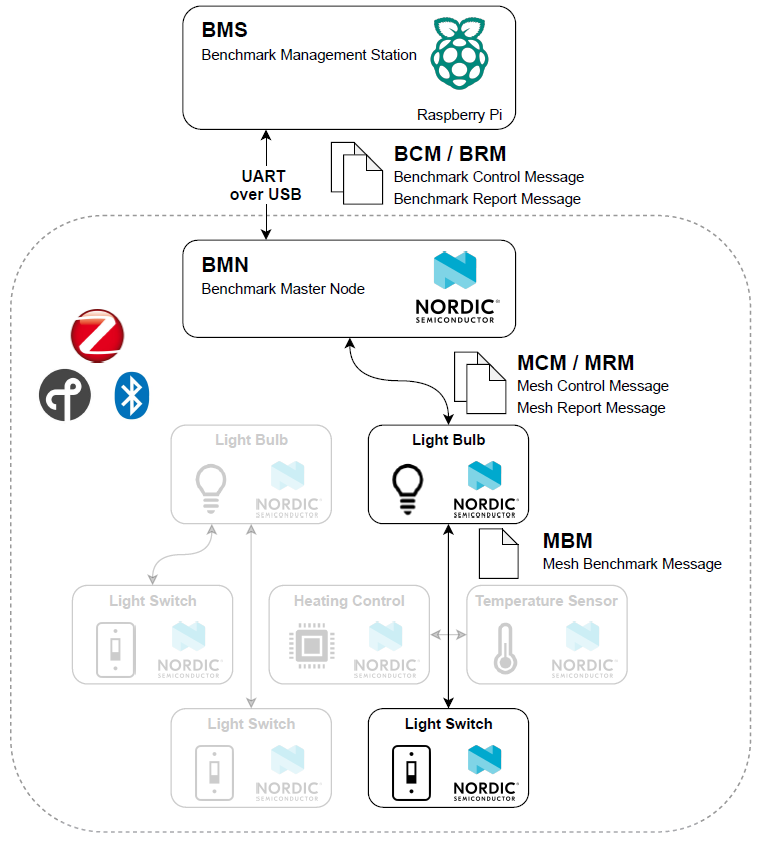
\includegraphics[width=1.0\textwidth]{Mesh_Testkonzept.png}
	\caption{Konzeptschema für den Ablauf eines Mesh Benchmarks.}\label{fig:MeshTestKonzept}
\end{figure}


\todo[inline]{RAN: Beschreibung Graphik einfügen}

\subsection{Mesh Benchmark Message (MBM)}\label{subsec:MeshBenchmarkMessage}
Die MBM ist jene Message welche die eigentlichen Messdaten produziert und diese sogleich unter den BSN (Mesh Knoten) überträgt. Anhand dieser Message werden die Parameter gemäss der Kennwerttabelle in Anhang xx erfasst.

\todo[inline]{Achtung Dummy Bild ;-)}

\begin{figure}[H]
	\centering
	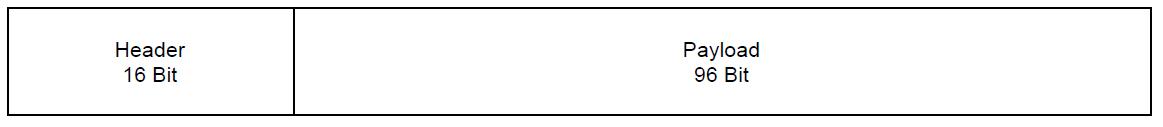
\includegraphics[width=1.0\textwidth]{MeshBenchmarkMessagePaketdefinition.png}
	\caption{Packet Definition der Mesh Benchmark Message (MBM)}\label{fig:MeshTestKonzept}
\end{figure}


\subsection{Mesh Control Message (MCM)}\label{subsec:MeshControlMessage}


\todo[inline]{Achtung Dummy Bild ;-)}

\begin{figure}[H]
	\centering
	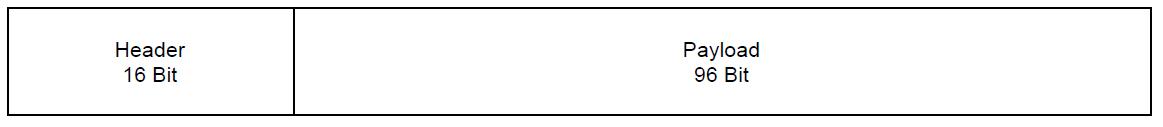
\includegraphics[width=1.0\textwidth]{MeshControlMessagePaketdefinition.png}
	\caption{Packet Definition der Mesh Control Message (MCM)}\label{fig:MeshTestKonzept}
\end{figure}

\subsection{Mesh Report Message (MRM)}\label{subsec:MeshReportMessage}


\todo[inline]{Achtung Dummy Bild ;-)}

\begin{figure}[H]
	\centering
	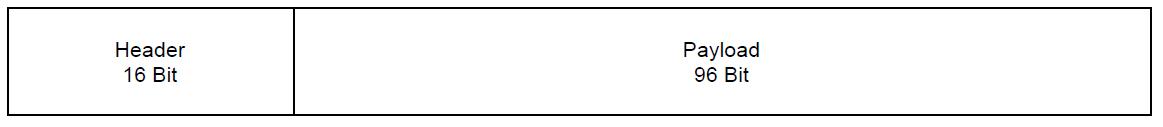
\includegraphics[width=1.0\textwidth]{MeshReportMessagePaketdefinition.png}
	\caption{Packet Definition der Mesh Report Message (MRM))}\label{fig:MeshTestKonzept}
\end{figure}

\subsection{Benchmark Control Message (BCM)}\label{subsec:BenchmarkControlMessage}

\todo[inline]{Achtung Dummy Bild ;-)}

\begin{figure}[H]
	\centering
	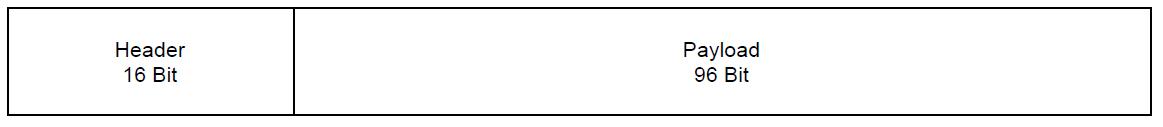
\includegraphics[width=1.0\textwidth]{BenchmarkControlMessagePaketdefinition.png}
	\caption{Packet Definition der Benchmark Control Message (BCM)}\label{fig:MeshTestKonzept}
\end{figure}

\subsection{Benchmark Report Message (BRM)}\label{subsec:BenchmarkReportMessage}

\todo[inline]{Achtung Dummy Bild ;-)}

\begin{figure}[H]
	\centering
	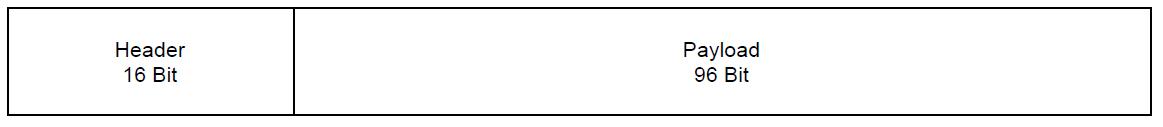
\includegraphics[width=1.0\textwidth]{BenchmarkReportMessagePaketdefinition.png}
	\caption{Packet Definition der Benchmark Report Message (BRM)}\label{fig:MeshTestKonzept}
\end{figure}



\pagebreak

	\clearpage
\section{Ablauf}\label{sec:Ablauf}
Ein Mesh Benchmark folgt einem klar definierten Ablauf. Die Abbildung \ref{fig:MeshTestkablauf} beschreibt den konzeptionellen Ablauf unabhängig vom zu testenden Mesh Protokoll.

\begin{figure}[H]
	\centering
	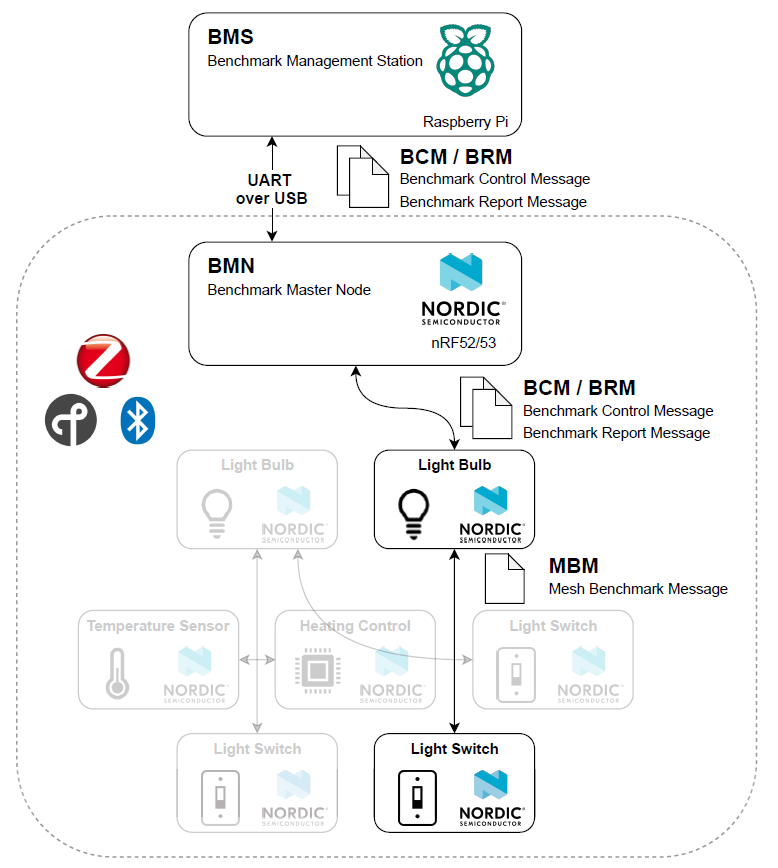
\includegraphics[width=1.0\textwidth]{Mesh_Testablauf.png}
	\caption{Konzeptschema für den Ablauf eines Mesh Benchmarks.}\label{fig:MeshTestkablauf}
\end{figure}

\begin{enumerate}
	\item \textbf{Benchmark User-Init:}\\
	Auf dem Webinterface des BMS werden die gewünschten Parameter definiert und der Benchmark durch den Benutzer gestartet.
	\item \textbf{Benchmark Init BMN:}\\
	Die Parameter werden an den BMN übergeben welcher diese wiederum an alle teilnehmenden BSN weiterleitet. Mit einem Startsignal vom BMN wird der Benchmark auf den BSN gestartet.
	\item \textbf{Benchmark Prozess:}\\
	Die BSN führen den Benchmark Prozess mit den definierten Parametern aus. Dies geschieht autonom und jeweils nur zwischen den entsprechenden BSN die in einer direkten Beziehung zueinander stehen (siehe Mesh Beziehungen \ref{subsec:MeshBeziehungen}). Die entstehenden Messdaten werden auf den BSN zwischen gespeichert.
	\item \textbf{Reporting:}\\
	Nach Ablauf der Benchmark Zeit werden die Messdaten an den BMN übertragen. Dies erfolgt gesteuert durch den BMN welcher die Daten bei einem BSN nach dem anderen abfragt und direkt an das BMS weiterleitet.
	\item \textbf{Finish:}\\
	Der BMN kontrolliert ob er die Daten von sämtlichen BSN korrekt auslesen konnte und bestätigt das Ende der Messung gegenüber dem BMS.
	\item \textbf{Auswertung:}\\
	Das BMS beendet den Benchmark Vorgang, speichert die Messdaten in seiner Datenbank ab und bereitet diese grafisch auf. 
\end{enumerate}









\pagebreak

	\clearpage
\section{Testszenarien}\label{sec:Testszenarien}

Die Benchmarks der Mesh Protokolle sollen mit unterschiedlichen Bedingungen getestet werden wobei grundsätzlich eine reelle Anwendung nachgebaut werden soll. Zum einen gibt es unterschiedliche Beziehungen innerhalb des Mesh Netzwerks, zum anderen werden Testumgebungen unterschieden.

\subsection{Mesh Beziehungen}\label{subsec:MeshBeziehungen}

Innerhalb eines Mesh Netzwerks können 4 Beziehungen zwischen den Nodes für die Benchmarks unterschieden werden. Üblicherweise kommen mehrere oder sogar alle 4 Beziehungen innerhalb eines Netzwerkes gleichzeitig zum Einsatz. Abbildung \ref{fig:MeshTestBeziehungen} zeigt die Beziehungen.

\begin{itemize}
 	\item \textcolor{red}{Rot stellt eine einfache P2P Verbindung ohne Hop dar. Beispielweise schaltet ein einzelner Schalter eine einzelne, definierte Lichtquelle}
 	\item \textcolor{orange}{Orange ist eine many-to-one Verbindung in welcher mehrere Lichtschalter die selbe Lichtquelle schalten.}
 	\item \textcolor{cyan}{In blau ist eine klassiche one-to-many Topologie dargestellt in welcher beispielsweise ein Schalter mehrere Lichtquellen bedient.}
 	 \item \textcolor{green}{Grün dargestellt ist eine indirekte P2P Verbindung mit. Das bedeutet, dass Schalter und Lichtquelle keine direkte Verbindung zueinander haben und daher Mesh-typisch via einem oder mehreren Hops kommuniziert.}
\end{itemize}

\begin{figure}[H]
	\centering
	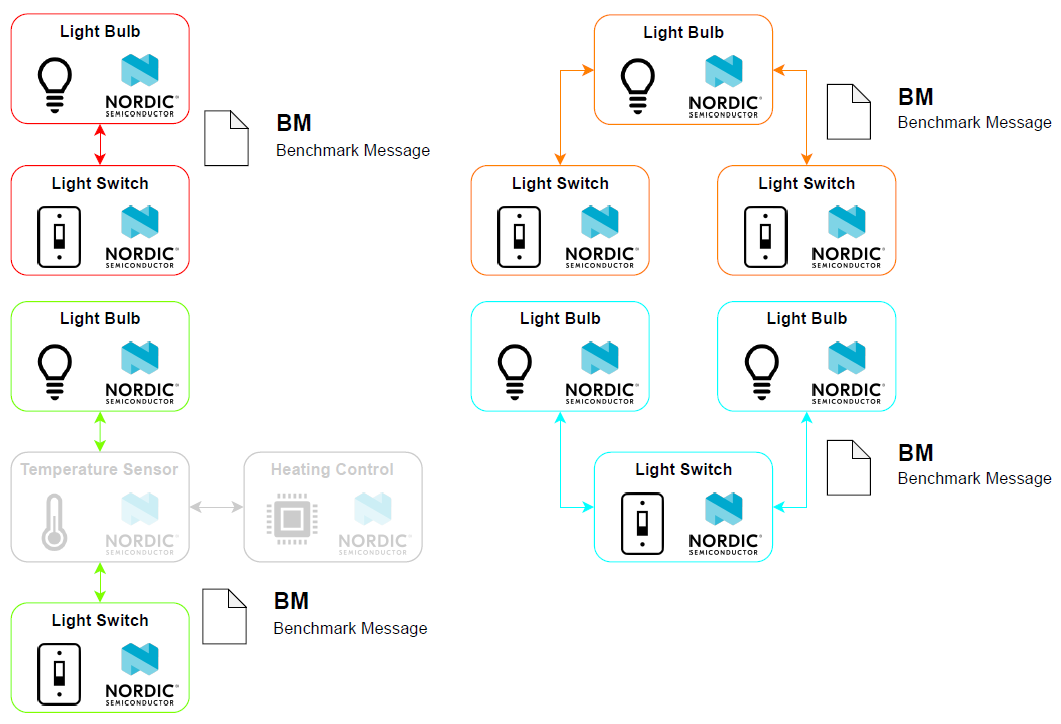
\includegraphics[width=1.0\textwidth]{Mesh_Test_Beziehungen.png}
	\caption{Beziehungen zwischen den Mesh Nodes innerhalb eines Benchmarks.}\label{fig:MeshTestBeziehungen}
\end{figure}


\subsection{Testumgebungen}\label{subsec:Testumgebungen}

Unterschiedliche Testumgebungen sollen die Benchmarks und schlussendlich den Vergleich der 3 Mesh Protokolle aussagekräftiger machen. Abbildung \ref{fig:MeshNetzwerkTestumgebungen} zeigt 5 unterschiedliche Umgebungen in denen Messungen durchgeführt werden sollen.

\begin{figure}[H]
	\centering
	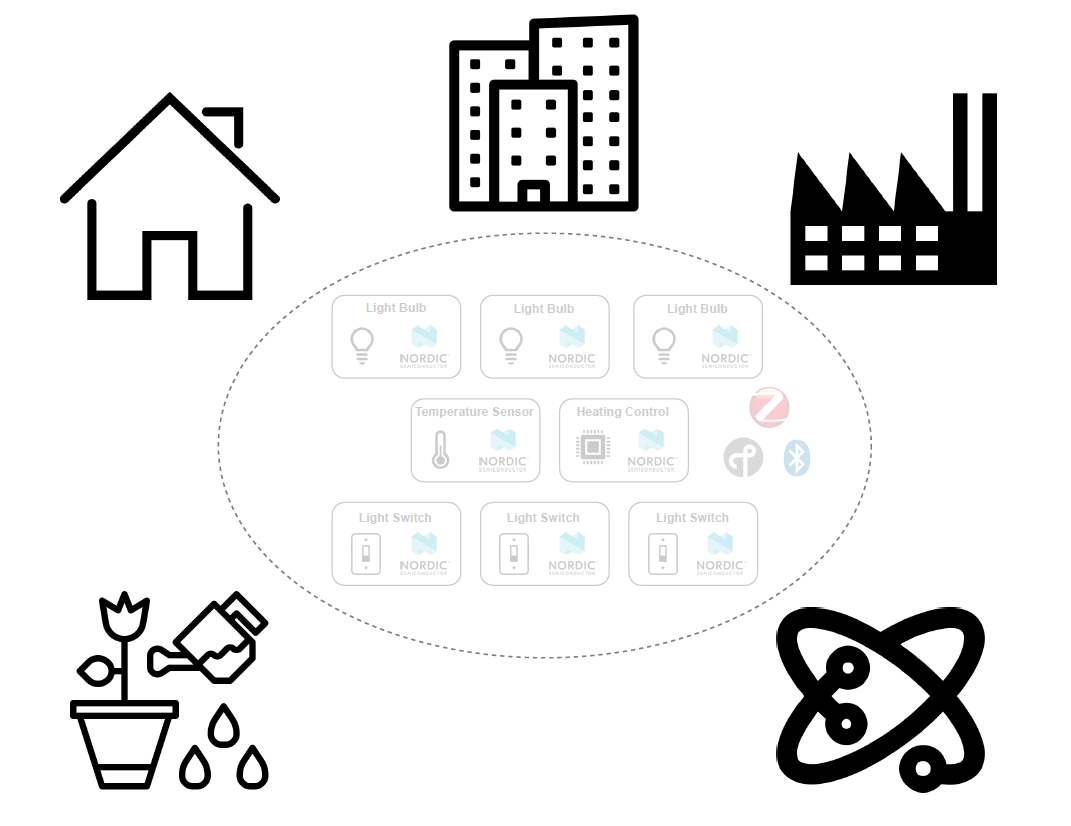
\includegraphics[width=1.0\textwidth]{Mesh_Testumgebung.png}
	\caption{Mesh Netzwerk Testumgebungen}\label{fig:MeshNetzwerkTestumgebungen}
\end{figure}

\begin{description}
\item[Haus] Die Testgeräte werden in einem Einfamilienhaus installiert und repräsentieren damit eine flächendeckende Heim-Automatisierung.
	\begin{itemize}
		\item Einfamilienhaus über mehrere Etagen.
		\item Anzahl Sensoren und Aktoren vergleichbar gross.
		\item Node-Dichte relativ gering.
		\item Keine Beeinflussung durch Nachbarsysteme zu erwarten \hfill \\
	\end{itemize}
\item[Wohnung] Ebenfalls als Heim-Automatisierung gedacht werden die Messungen in einer Wohnung durchgeführt.
	\begin{itemize}
		\item Wohnung über eine Etage in einem Mehrfamilienhaus
		\item Anzahl Sensoren und Aktoren vergleichbar gross.
		\item Node-Dichte höher als im Haus.
		\item Mögliche Störeinflüsse durch andere Systeme von Nachbarn zu 					erwarten. \hfill \\
	\end{itemize}
\item[Industrie] Um eine Industrielle Anwendung zu vergleichen erfolgt eine Messung in einem Industriebetrieb.
	\begin{itemize}
		\item Industriebetrieb mit grosser Fläche.
		\item Grosse Anzahl Sensoren zur Überwachung von Produktionsprozessen. 				Vereinzelt Aktoren zur Ansteuerung von Anlageteilen.
		\item Hohe Node-Dichte.
		\item Mögliche Störeinflüsse durch Maschinen oder Abschirmwirkung durch 			metallische Gegenstände zu erwarten. \hfill \\
	\end{itemize}
\item[Landwirtschaft (optional)] Für die Überwachung und Kontrolle von landwirtschaftlichen Flächen kann ein Test auf offenem Feld erfolgen.
	\begin{itemize}
		\item Landwirtschaftsfläche mit grosser Ausbreitung (z.B. Gemüseanbau).
		\item Grosse Anzahl Sensoren. Nur wenige bis gar keine Aktoren.
		\item Sehr geringe Node-Dichte mit weiten Distanzen.
		\item Geringe bis keine Störbeeinflussung durch die Umgebung zu erwarten. \hfill \\
	\end{itemize}
\item[Labor] Der Laboraufbau ist ein Extremtest welcher die Leistungsgrenzen der Protokollstacks ausloten soll.
	\begin{itemize}
		\item Testaufbau unter Laborbedingungen auf engstem Raum.
		\item Ausgeglichene Anzahl Sensoren und Aktoren.
		\item Sehr Hohe Node-Dichte.
		\item Geringe bis keine Störbeeinflussung durch die Umgebung zu erwarten. \hfill \\
	\end{itemize} 
\end{description}







\pagebreak

	\clearpage
\section{Firmware}\label{sec:Firmware}

\todo[inline]{Eine Hardwareplattform. Dongle mit Akku für die BSN und DK für den BMN. Firmware dementsprechend gibt es folgende: BMN, BSN Sensor, BSN Aktor}

\todo[inline]{Räffu: Mesh-5, 7, 8, 9}
\todo[inline]{Robin: Mesh-1, 3, 4}
\todo[inline]{Robin: Mesh-2, 6, 10}


\subsection{Parameter Mesh Test}\label{subsec:ParameterMeshTest}




\pagebreak

	\clearpage
\section{Hardware}\label{sec:Hardware}

\todo[inline]{Eine Hardwareplattform. Dongle mit Akku für die BSN und DK für den BMN. Firmware dementsprechend gibt es folgende: BMN, BSN Sensor, BSN Aktor}






\pagebreak



\clearpage
%%---BIBLIOGRAPHY------------------------------------------------------------------------
{\sloppypar
\printbibliography[heading=bibintoc]
\label{sec:lit}
%\selectlanguage{ngerman}				%ngerman or english
%\printbibliography
}

%%---APPENDIX----------------------------------------------------------------------------
\begin{appendix} 

\addcontentsline{toc}{section}{Anhang}


%**********************Aufgabenstellung***************************
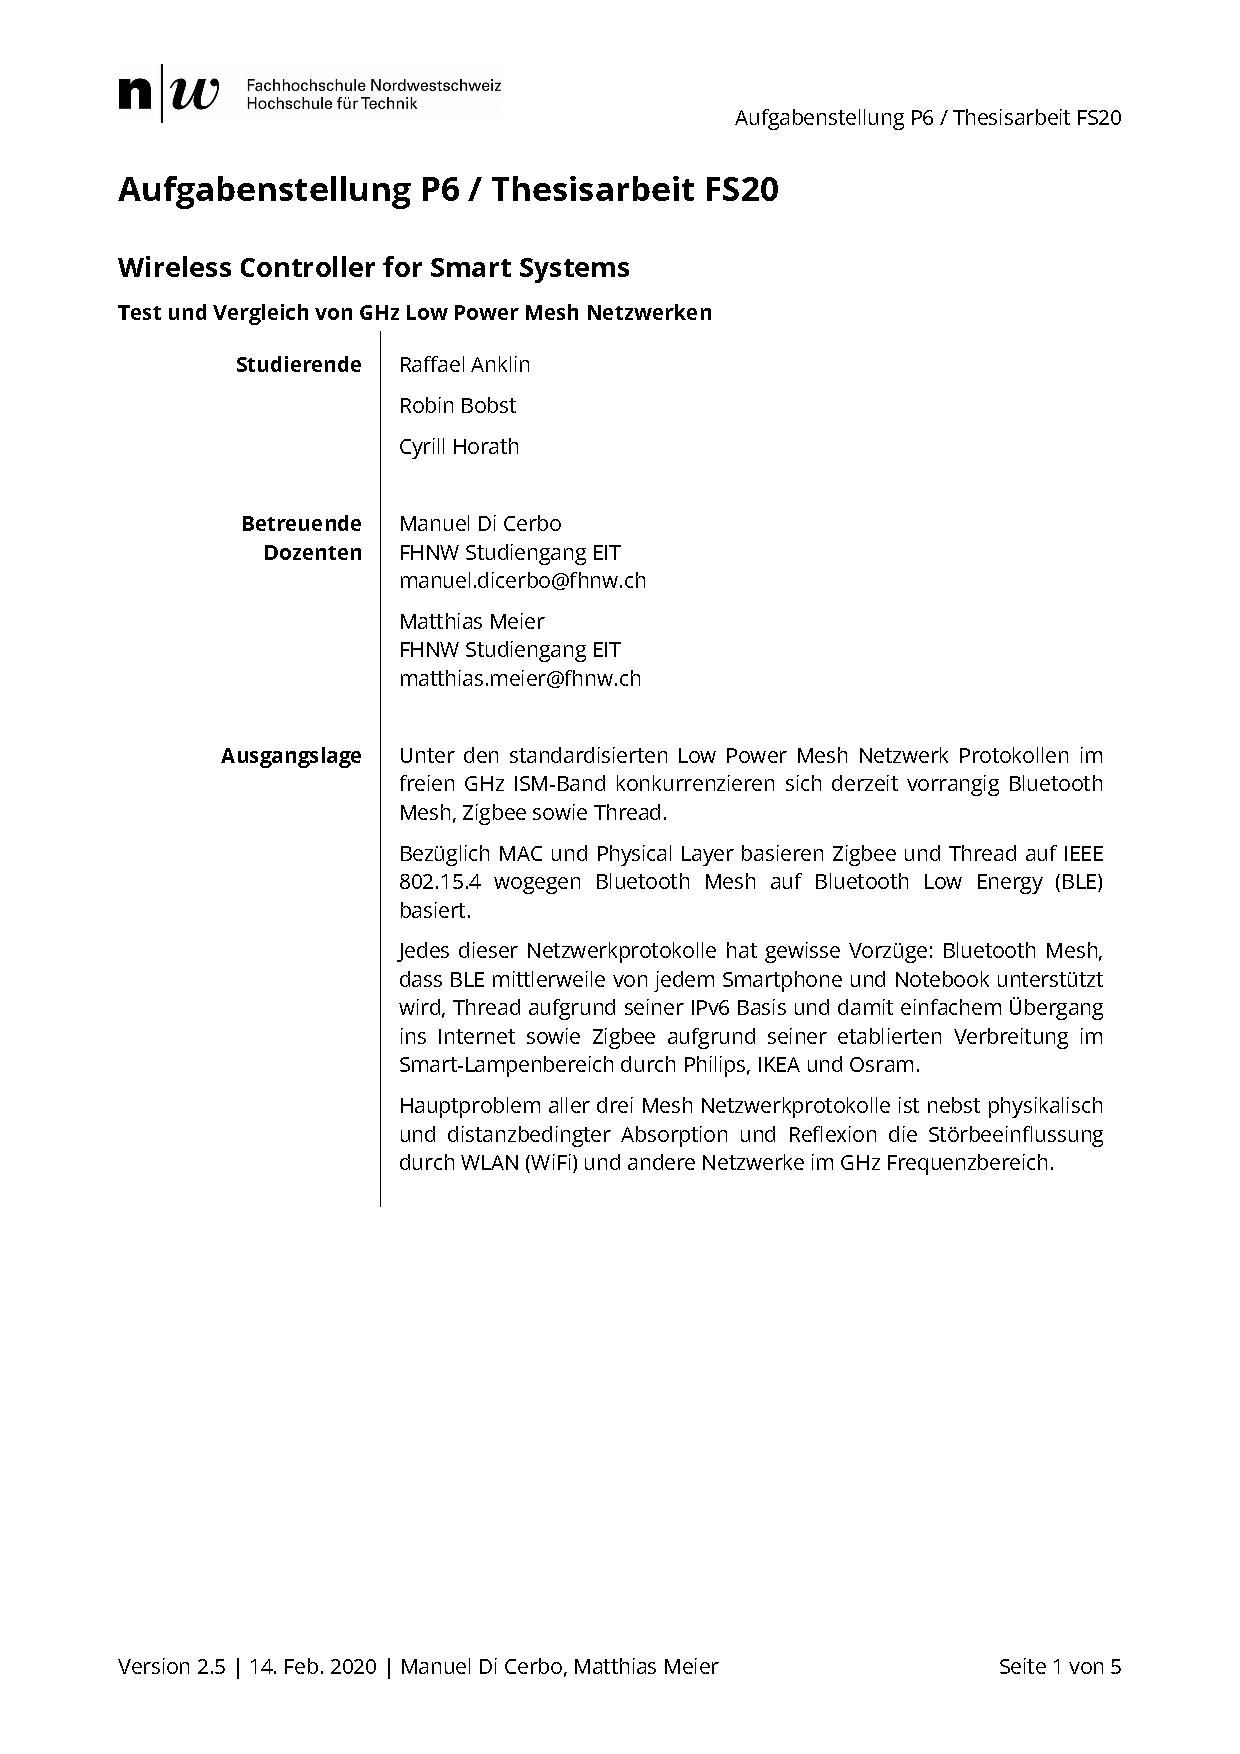
\includepdf[pages={1}, nup=1x1, landscape=false, scale=0.9 ,offset=0 -45, pagecommand={\section{Aufgabenstellung}\label{app:Aufgabenstellung}\thispagestyle{myheadings}}]{appendix/P6_Aufgabenstellung_Wireless_Controller_for_Smart_Systems.pdf}

\includepdf[pages={2-5}, nup=1x1, landscape=false, scale=0.9 ,offset=0 -45, pagecommand={\thispagestyle{myheadings}}]{appendix/P6_Aufgabenstellung_Wireless_Controller_for_Smart_Systems.pdf}


%**********************Pflichtenheft***************************

\includepdf[pages={1}, nup=1x1, landscape=false, scale=0.95 ,offset=0 -45, pagecommand={\section{Pflichtenheft}\label{app:Pflichtenheft}\thispagestyle{myheadings}}]{appendix/P6_Pflichtenheft.pdf}


\includepdf[pages={2-19}, nup=1x1, landscape=false, scale=0.95 ,offset=0 -45, pagecommand={\thispagestyle{myheadings}}]{appendix/P6_Pflichtenheft.pdf}

%***************EMV Bericht Abstrahlung Antennen*********************
\includepdf[pages={1}, nup=1x1, landscape=false, scale=0.95 ,offset=0 -45, pagecommand={\section{Bericht emv Messung Development Kits}\label{app:BerichtemvMessungDevelopmentKits}\thispagestyle{myheadings}}]{appendix/emv_Bericht_FS20.pdf}

\includepdf[pages={2-13}, nup=1x1, landscape=false, scale=0.95 ,offset=0 0, pagecommand={\thispagestyle{myheadings}}]{appendix/emv_Bericht_FS20.pdf}

%***************Messprotokolle Mesh Benchmark*********************
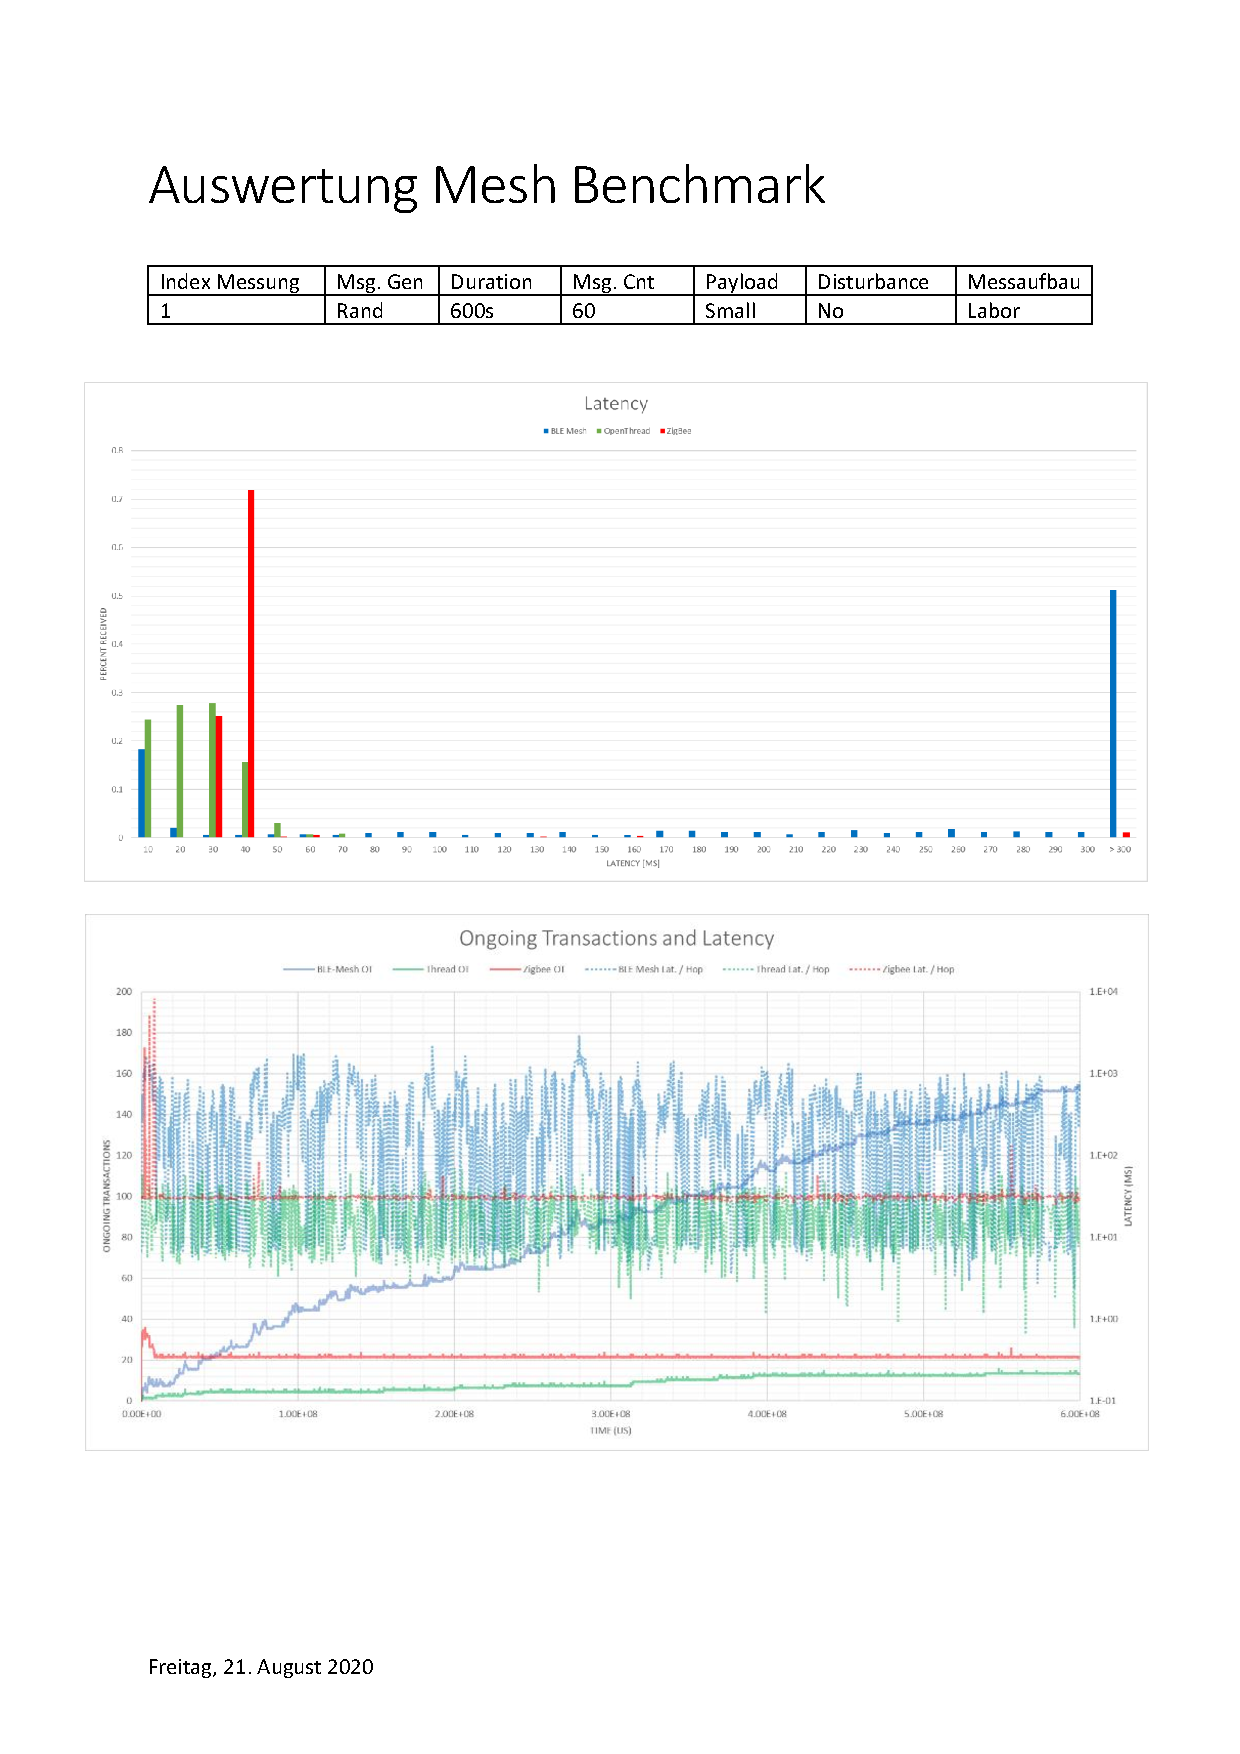
\includepdf[pages={1}, nup=1x1, landscape=false, scale=0.95 ,offset=0 -20, pagecommand={\section{Messprotokolle Mesh Benchmark}\label{app:MessprotokolleMeshBenchmark}\thispagestyle{myheadings}}]{appendix/Messprotokolle_Labor.pdf}

\includepdf[pages={2-14}, nup=1x1, landscape=false, scale=0.95 ,offset=0 0, pagecommand={\thispagestyle{myheadings}}]{appendix/Messprotokolle_Labor.pdf}

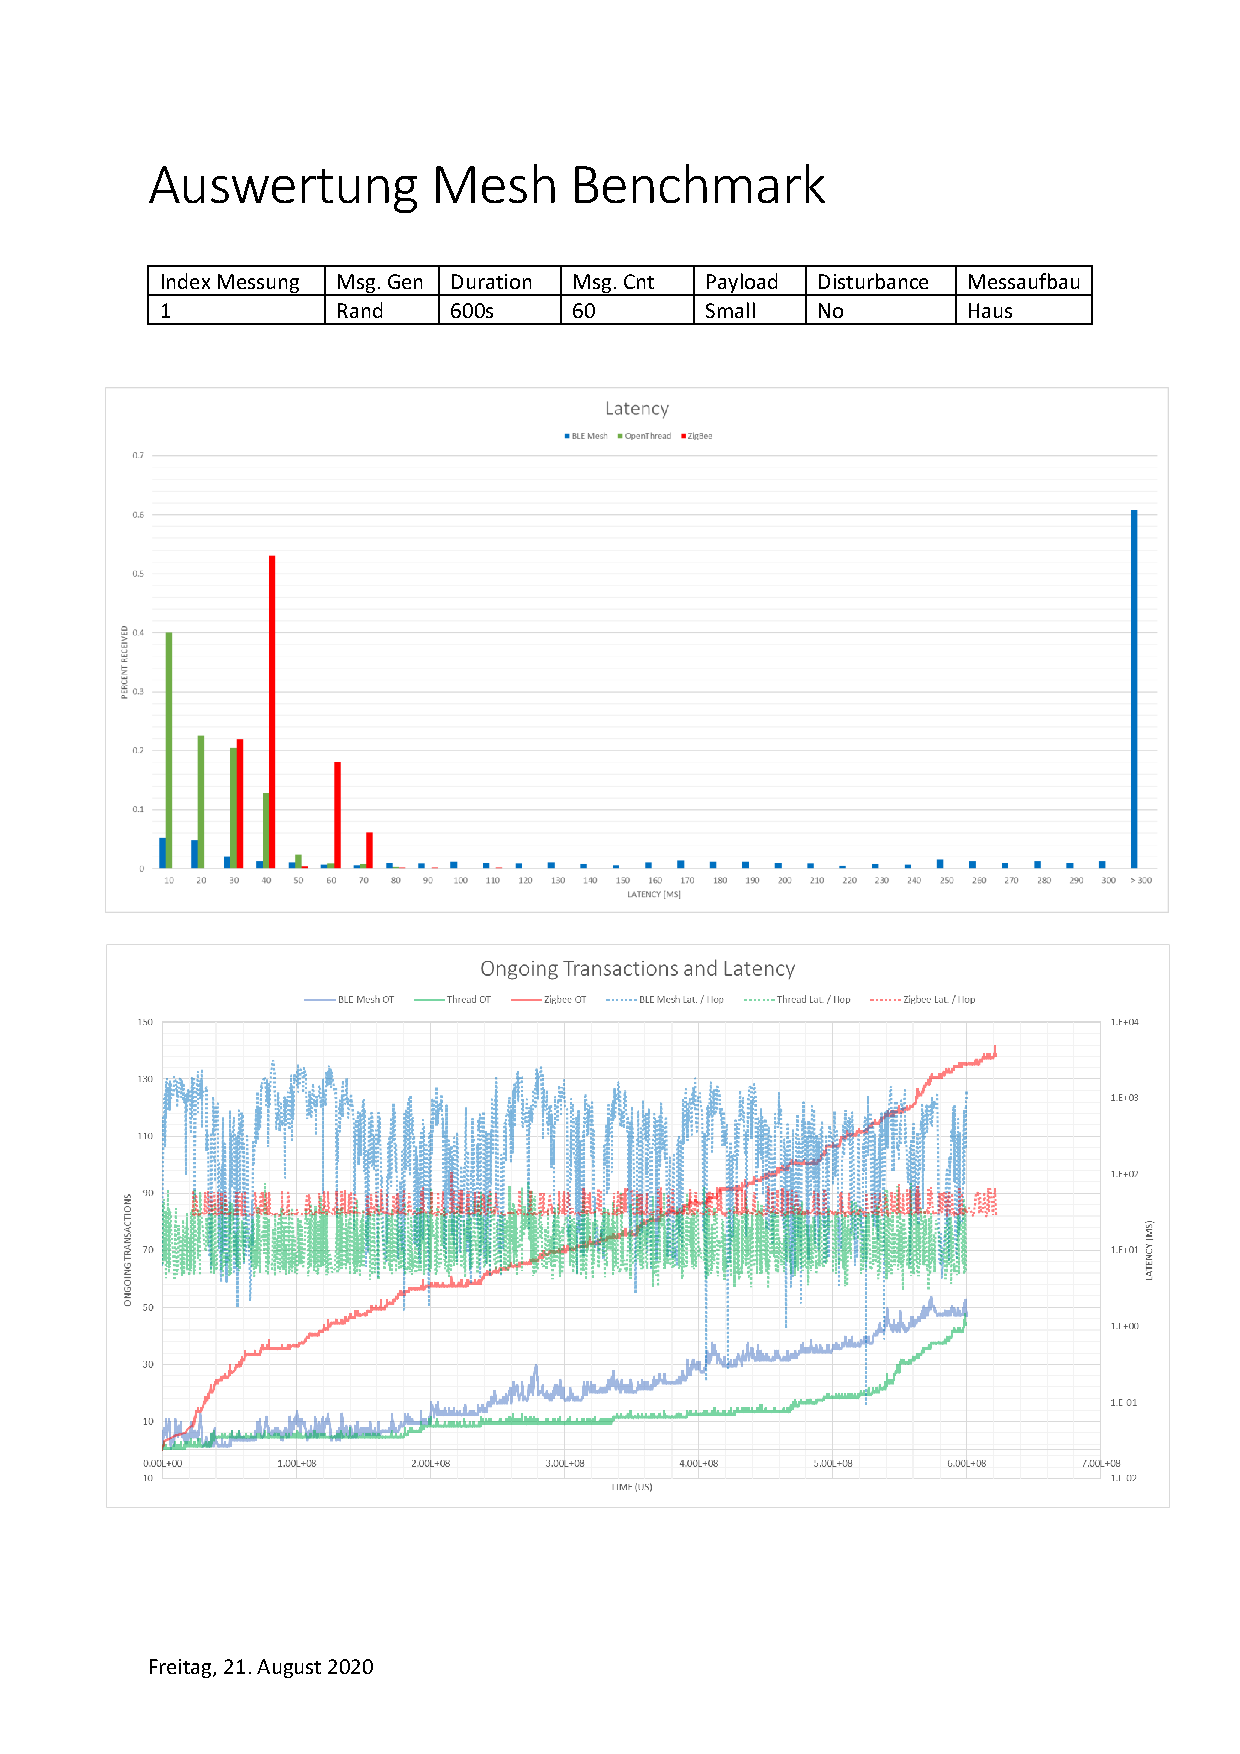
\includepdf[pages={1}, nup=1x1, landscape=false, scale=0.95 ,offset=0 0, pagecommand={\thispagestyle{myheadings}}]{appendix/Messprotokolle_Haus.pdf}

\includepdf[pages={2-8}, nup=1x1, landscape=false, scale=0.95 ,offset=0 0, pagecommand={\thispagestyle{myheadings}}]{appendix/Messprotokolle_Haus.pdf}

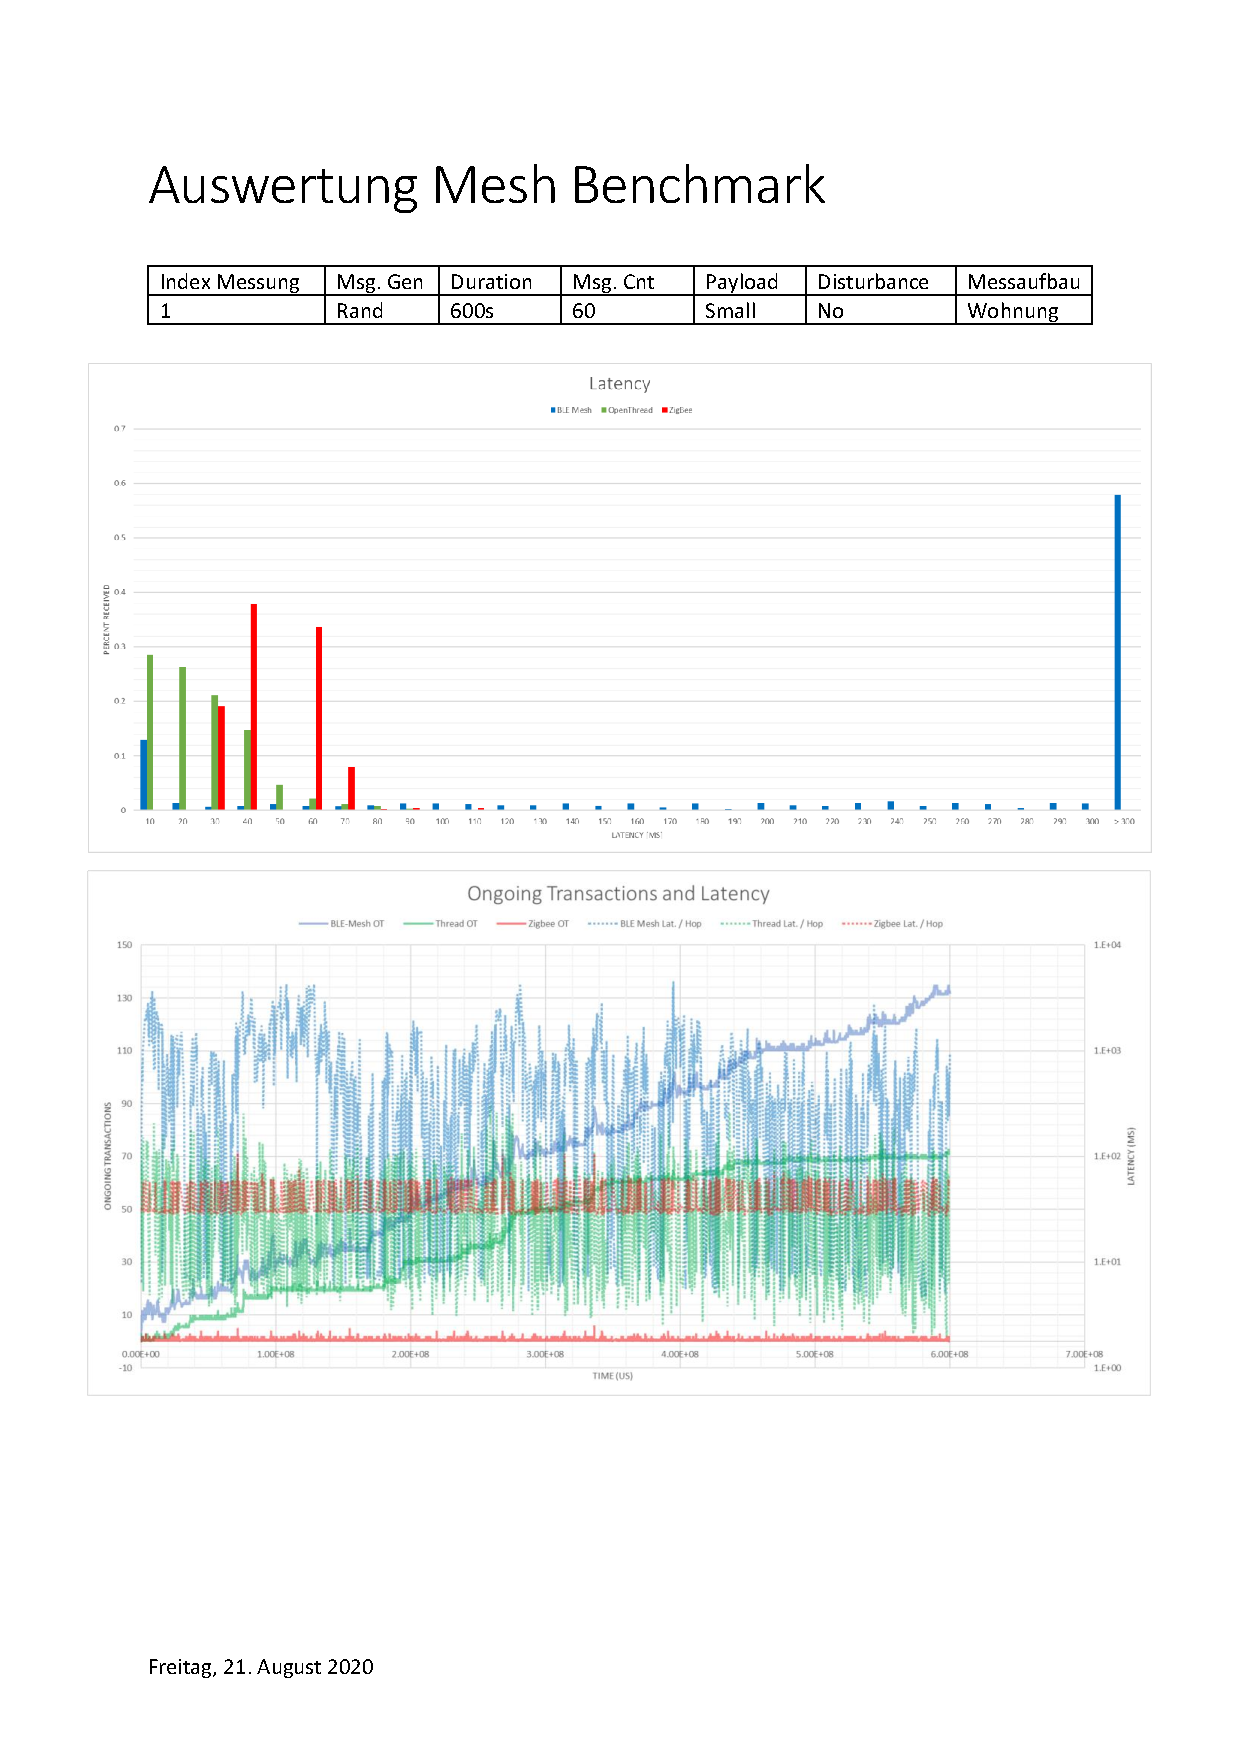
\includepdf[pages={1}, nup=1x1, landscape=false, scale=0.95 ,offset=0 0, pagecommand={\thispagestyle{myheadings}}]{appendix/Messprotokolle_Wohnung.pdf}

\includepdf[pages={2-8}, nup=1x1, landscape=false, scale=0.95 ,offset=0 0, pagecommand={\thispagestyle{myheadings}}]{appendix/Messprotokolle_Wohnung.pdf}

%***************Random Value Generation*********************
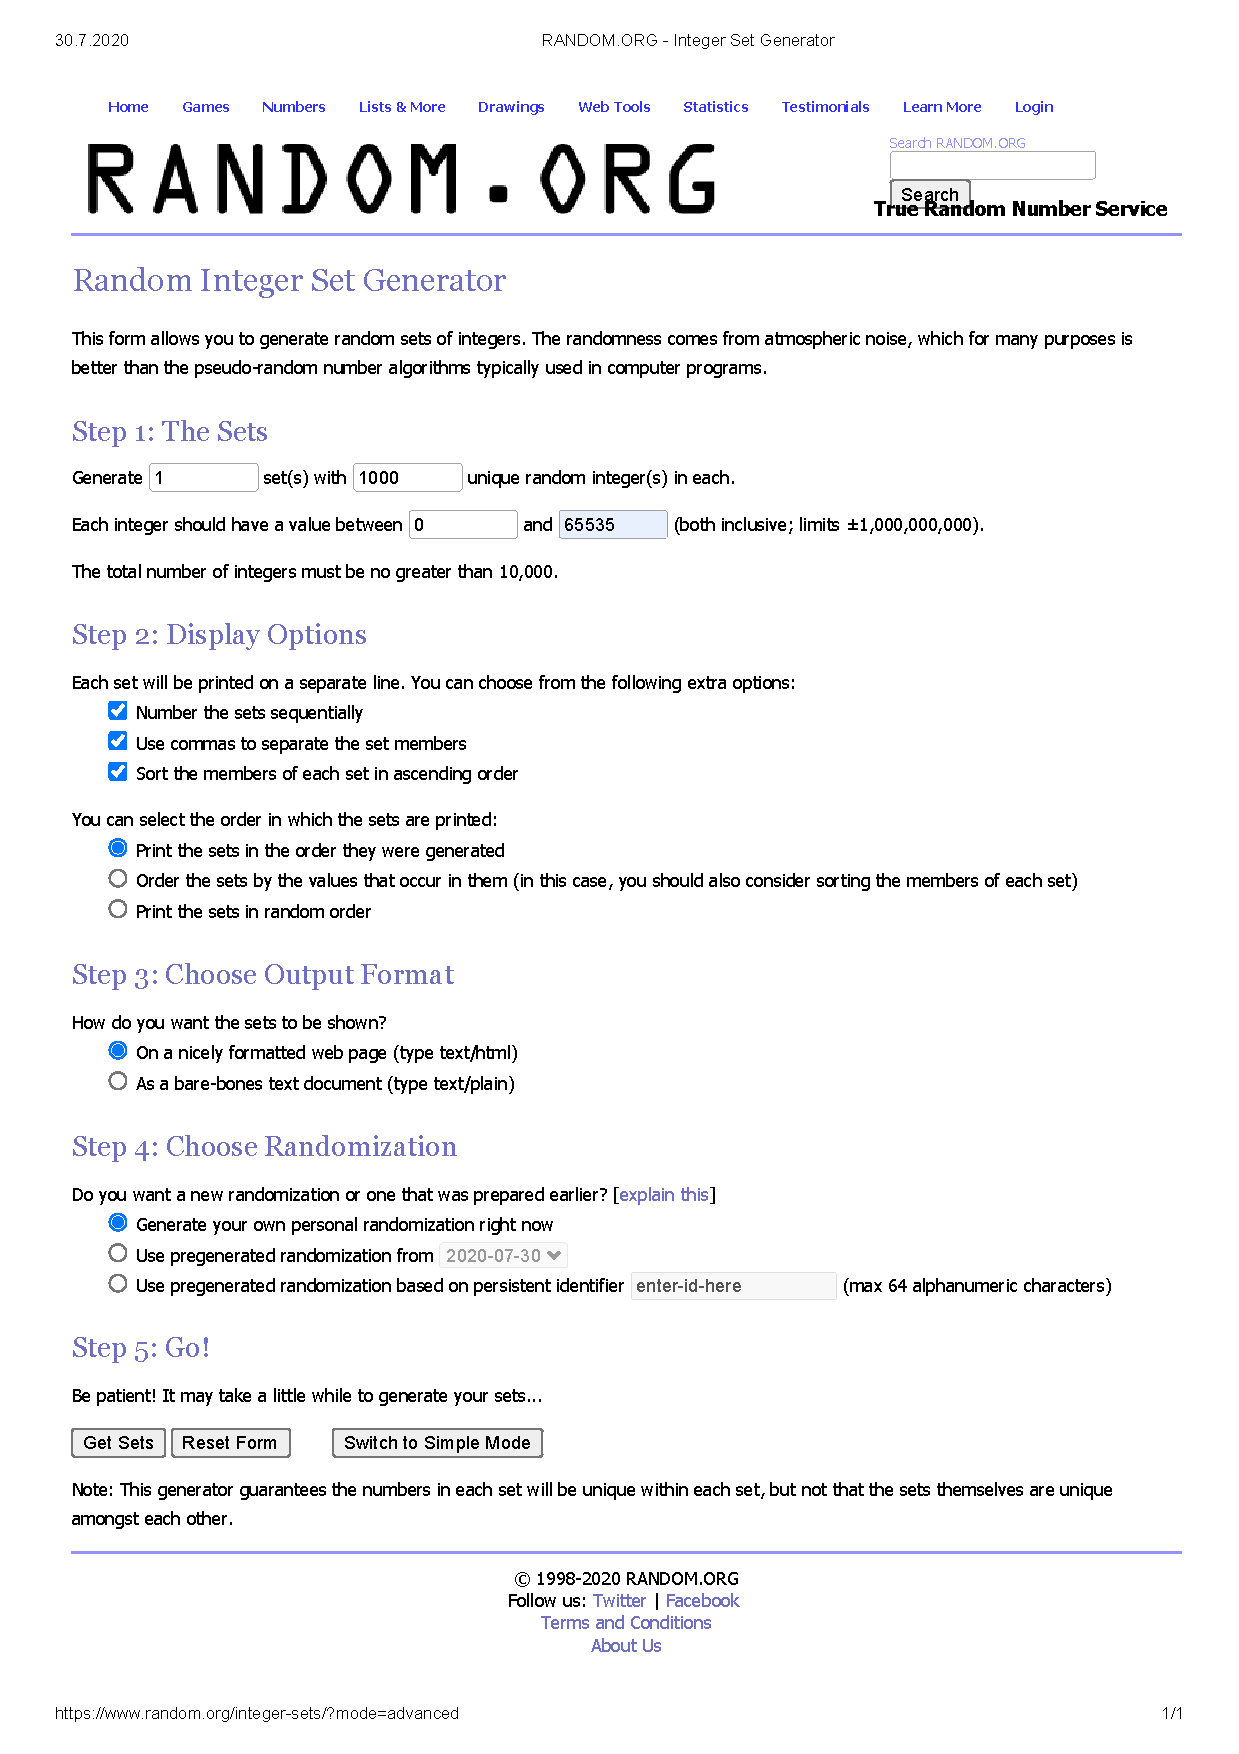
\includepdf[pages={1}, nup=1x1, landscape=false, scale=0.8 ,offset=0 -20, pagecommand={\section{Random Traffic Generation}\label{app:RandomTrafficGeneration}\thispagestyle{myheadings}}]{appendix/RANDOM.ORG_Integer_Set_Generator.pdf}


\end{appendix}



%%---NOTES for DEBUG---------------------------------------------------------------------
\ifdraft{%Do this only if mode=draft
%%requires \usepackage{todonotes})
\newpage
\listoftodos[\section{Todo-Notes}]
\clearpage
}
{%Do this only if mode=final
}

\end{document}
